\documentclass[10pt,conference,letterpaper]{IEEEtran}
\usepackage{times,amsmath,epsfig}
\usepackage{algorithm}
\usepackage{algorithmic}
\usepackage{graphicx}
%\usepackage{epsfig}
\usepackage{color}
\usepackage{amssymb}
%\usepackage{amsmath}
\usepackage{flushend}
\usepackage{cite,float}
\usepackage[normalem]{ulem}
\usepackage{verbatim}
%\usepackage{subfig}
\usepackage{subfigure}

\title{Anonymous Network Protocol for Mobile Participatory Sensing}

\author{
Chih-Jye Wang, Wei-Shinn Ku, John Patrick Wall
% add some space between author names and affils
\vspace{1.6mm}\\
\fontsize{10}{10}\selectfont\itshape
Department of Computer Science and Software Engineering\\
Auburn University, AL, USA\\
\fontsize{9}{9}\selectfont\ttfamily\upshape
\{wangchj, wzk0004, jpw0001\}@auburn.edu\\
}

\begin{document}

\maketitle

\begin{abstract}
In the participatory sensing, users with mobile devices (e.g. cell phones
and laptop computers) participate in the collection of environmental
information around them and submit the collected data to a central server
for processing and analysis. Identity privacy of mobile users in this model
is a major concern that hinders the adoption of this computing model. In
this paper, we propose an anonymous networking protocol approach to protect
the identity of participants of such computing model.
\end{abstract}

% NOTE keywords are not used for conference papers so do not populate them
\begin{keywords}
ignore
\end{keywords}
%


In participatory
sensing~\cite{conf/sensys/ReddyBEHS07,conf/sensys/DuttaAKMMWW09},
users with mobile devices (e.g., cell phones with GPS chips)
participate in the collection of environmental information around
them and submit the collected data (image, audio, video, etc.) to
a central server for process, analysis, and
storage~\cite{DBLP:conf/mobisys/MunRSYBEHHWB09}. An example is the
OpenStreetMap~\cite{DBLP:journals/pervasive/HaklayW08} project,
which collects user contributed GIS data (such as GPS traces and
POIs) and constructs an online map, from mobile data, open for the
public to use. Other examples of participatory sensing include
cooperative collection of gas
prices~\cite{DBLP:conf/dcoss/DongKCB08}, monitoring of traffic
conditions~\cite{DBLP:conf/dcoss/ConceicaoFB08}, and photo sharing
through mobile applications such as Facebook and Instagram.

This model of ``crowd" data collection has many advantages due to
that the dynamic environmental data and information are quickly
captured by mobile users and disseminated to other users or to
central servers for analysis. Government censoring of information
is also less effective in this model since there could be many
mobile devices that are capturing the same event.

Despite the advantages, privacy of the users who contribute is a
major issue in participatory sensing and crowd-sourcing. Users may
not want to leak their locations with the contributed data lest
their movement should be
tracked~\cite{conf/icde/YiuJHL08,journals/pvldb/WangL09}. In the
case of controversial photos, a user may not want to reveal his or
her identity to the collection server (such as
WikiLeaks\footnote{http://wikileaks.org/}) since the user's
identity may be saved on the server and later uncovered by
government entities for prosecution. It is a fact that services on
the web collect user identifications along with the data submitted
by their users~\cite{wiki_privacy}. Even with websites, such as
Wikipedia\footnote{http://www.wikipedia.com} and
4chan\footnote{http://www.4chan.org/faq\#what4chan} that advertise
to be anonymous log IP addresses of contributors. Although an IP
address does not uniquely identify an individual, cellular data
service providers are required by law to keep record of assignment
of IP addresses to mobile users for a period of
time\footnote{http://uscode.house.gov/download/pls/18C121.txt}.
With an IP address, a piece of information stored on a server (be
it a photo, or a file) can be traced back to a user using the
technique discussed in~\cite{DBLP:journals/ijufks/Sweene02} thus
compromises the user's privacy.

How to guarantee that a service provider will not gather users'
identification? Many previous
works~\cite{DBLP:conf/uss/DingledineMS04,DBLP:journals/cacm/ReiterR99,
DBLP:journals/jcs/LevineS02} have addressed the issues of user
anonymity on the Internet. Unfortunately, most previously proposed
solutions are designed for the older computing model of desktop
computing where network bandwidth and computing power are not
major concerns. In mobile environments, both bandwidth and
computational capability are limited partially due to the size of
devices and battery power constraints.

In this paper, we propose an anonymous data sharing method with
constraints of mobile, participatory sensing environments in mind.
The goal is to design a solution that is simple so that it does
not consume to much resource for mobile devices (resources being
bandwidth and computational power), and at the same time provide
adequate protection for privacy. We want to keep the identity of
data owners (senders) private to various parties in a computer
network, especially to the data collection server (receiver) since
without identity information associated with submitted data on the
server, linking to data originator is difficult. Although we
mainly focus on keeping sender anonymous to the server, we believe
our solution has enough protection from other parties in a
network. Our mechanism is to remove the source information from
data packets. We call this One-Way Protocol since the source
information is completely removed, and the server is unable to
reply any kind of acknowledgement back to the client. The protocol
will be implemented on both the server and the client to achieve
the anonymous effect.

The rest of this paper is organized as follows. In
section~\ref{sec-related-works}, we survey previous works for
anonymity on data communication. For each work, we identify
strengths and weaknesses relative to our design goals. We present
our anonymous One-Way protocol in Section~\ref{sec-protocol}. We
discuss how data payload is transmitted and how uploaded data is
verified although the server does not know the identity of the
sender. Section~\ref{sec-imp} presents the implementation issues
and Section~\ref{sec-attack} discusses a few attack models. The
experimental validation of our design in
Section~\ref{sec-evaluation}. Section~\ref{sec-conc} concludes
this paper with a discussion of future work.

\section{Related Works}\label{sec-related-works}
One of the earliest work on anonymous communication is on untraceable
electronic mail by Chaum\cite{DBLP:journals/cacm/Chaum81}. The work proposed
a way of sending an electronic mail to a receiver in which the sender
remain anonymous using one or a series of proxy computers called Mixes.
Chaum's solution relies heavily on public key cryptography in a way that
before forwarding a mail to a mix, the message and the receiver's address
is encrypted using the mix's public key. Upon receiving an electronic
message, the mix extracts the information
and forwards the mail to the intended receiver. In the case of multiple
mixes, the sender performs one public key cryptography for each mixes before
sending a mail to the first mix. The mix then forward it to the next mix
and so on until the mail reaches the receiver. One of the drawback of the
solution proposed in \cite{DBLP:journals/cacm/Chaum81} is scalability since
the senders depend on fixed proxies and if there are not proxies, the
solution will not work. Also multiple public key cryptography is expensive
for mobile devices. Multiple public key is acceptable for small file, but
for large files that need to be broken down and sent with multiple segments,
multiple encryption may not be acceptable.

Another well known research of sender anonymity is the
onion routing\cite{DBLP:conf/uss/DingledineMS04}. The onion routing
follows the similar approach as in \cite{DBLP:journals/cacm/Chaum81} of
using multiple proxies and multiple encryptions. Before sending a file,
the sender selects a number of proxies called onion routers. The selected
routers have no say in the selection process, thus mitigating malicious
node collaboration attack. After selecting the routers, the sender
encrypts its data with the key of the first router, then encrypt the result
of that with the key of the second router, and does the same for all the
routers. Onion routing is robust in terms
of security and can be used in many applications, but it has the same
drawback as in Chaum's approach that it is computationally expensive
because of the multiple encryptions. Our solution does not impose multiple
encryption to the application, but give that choice to the developer
of the application.

Freenet, a distributed anonymous storage system was proposed
in \cite{DBLP:conf/diau/ClarkeSWH00}. The goal of the system is to utilize
the peers in the network for storage and at the same time achieving anonymity
of the author of the files. Freenet utilizes file keys obtained by public
key cryptography and hashing to achieve efficient file storage and searching.
In order to achieve author anonymity, a node on the Freenet sends a file
to a peer, and the peer forwards the file to another peer and so on, much
like the solution in Crowds. Although, the system pertains to file storage,
the technique of utilizing peers to hide the identity of the originator of
a file is useful in our scenario and we take a similar approach with our
data verification of our design.

Crowds\cite{DBLP:journals/cacm/ReiterR99} utilizes peer-to-peer network
to blend the sender into a large number of users (a crowd) so that the
receiver does not know the true identity of the sender.
To send a file, the sender joins a close-by crowd and sends the file to
one of its peers in the crowd called jondo (a short name for John Doe).
When a peer receives a send request, it decides whether to forward the
data to another peer based on the variable $p_f$ that determines the
probability of forwarding the packet.

The closest work to ours is research on privacy for mobile users in sensing
networks \cite{DBLP:conf/percom/HuS10} by Hu and Shahabi. The assumption of the
work is that data collection service providers often log the identity of the
user with the file they submit. The disclosure of this sensitive information
leads to the compromising of user privacy. The solution is to leverage
social network to forward a file to multiple peers before sending it to
the server. Large consumption of network bandwidth is a big disadvantage in
this approach since a file is sent to multiple users, and this concern is
exacerbated in wireless mobile environments where bandwidth is limited.
In our approach, we do not forward the payload of the data to multiple peers,
only the control messages of the data transmission and saves tremendous amount
of bandwidth.
\section{Anonymous Protocol}\label{sec-protocol}

In this section, we propose a way to protect the identity of participants
of such computing model by using a novel(?) anonymous networking protocol.
The goal of the protocol is to remove the source information from the data
packet. We call this One-Way Protocol since the source information is
complectly removed, and the server is unable to reply any kind of
acknowledgement back to the client. The protocol will be implemented on
both the server and the client to achieve the anonymous effect.

\begin{figure}[h]
\begin{center}
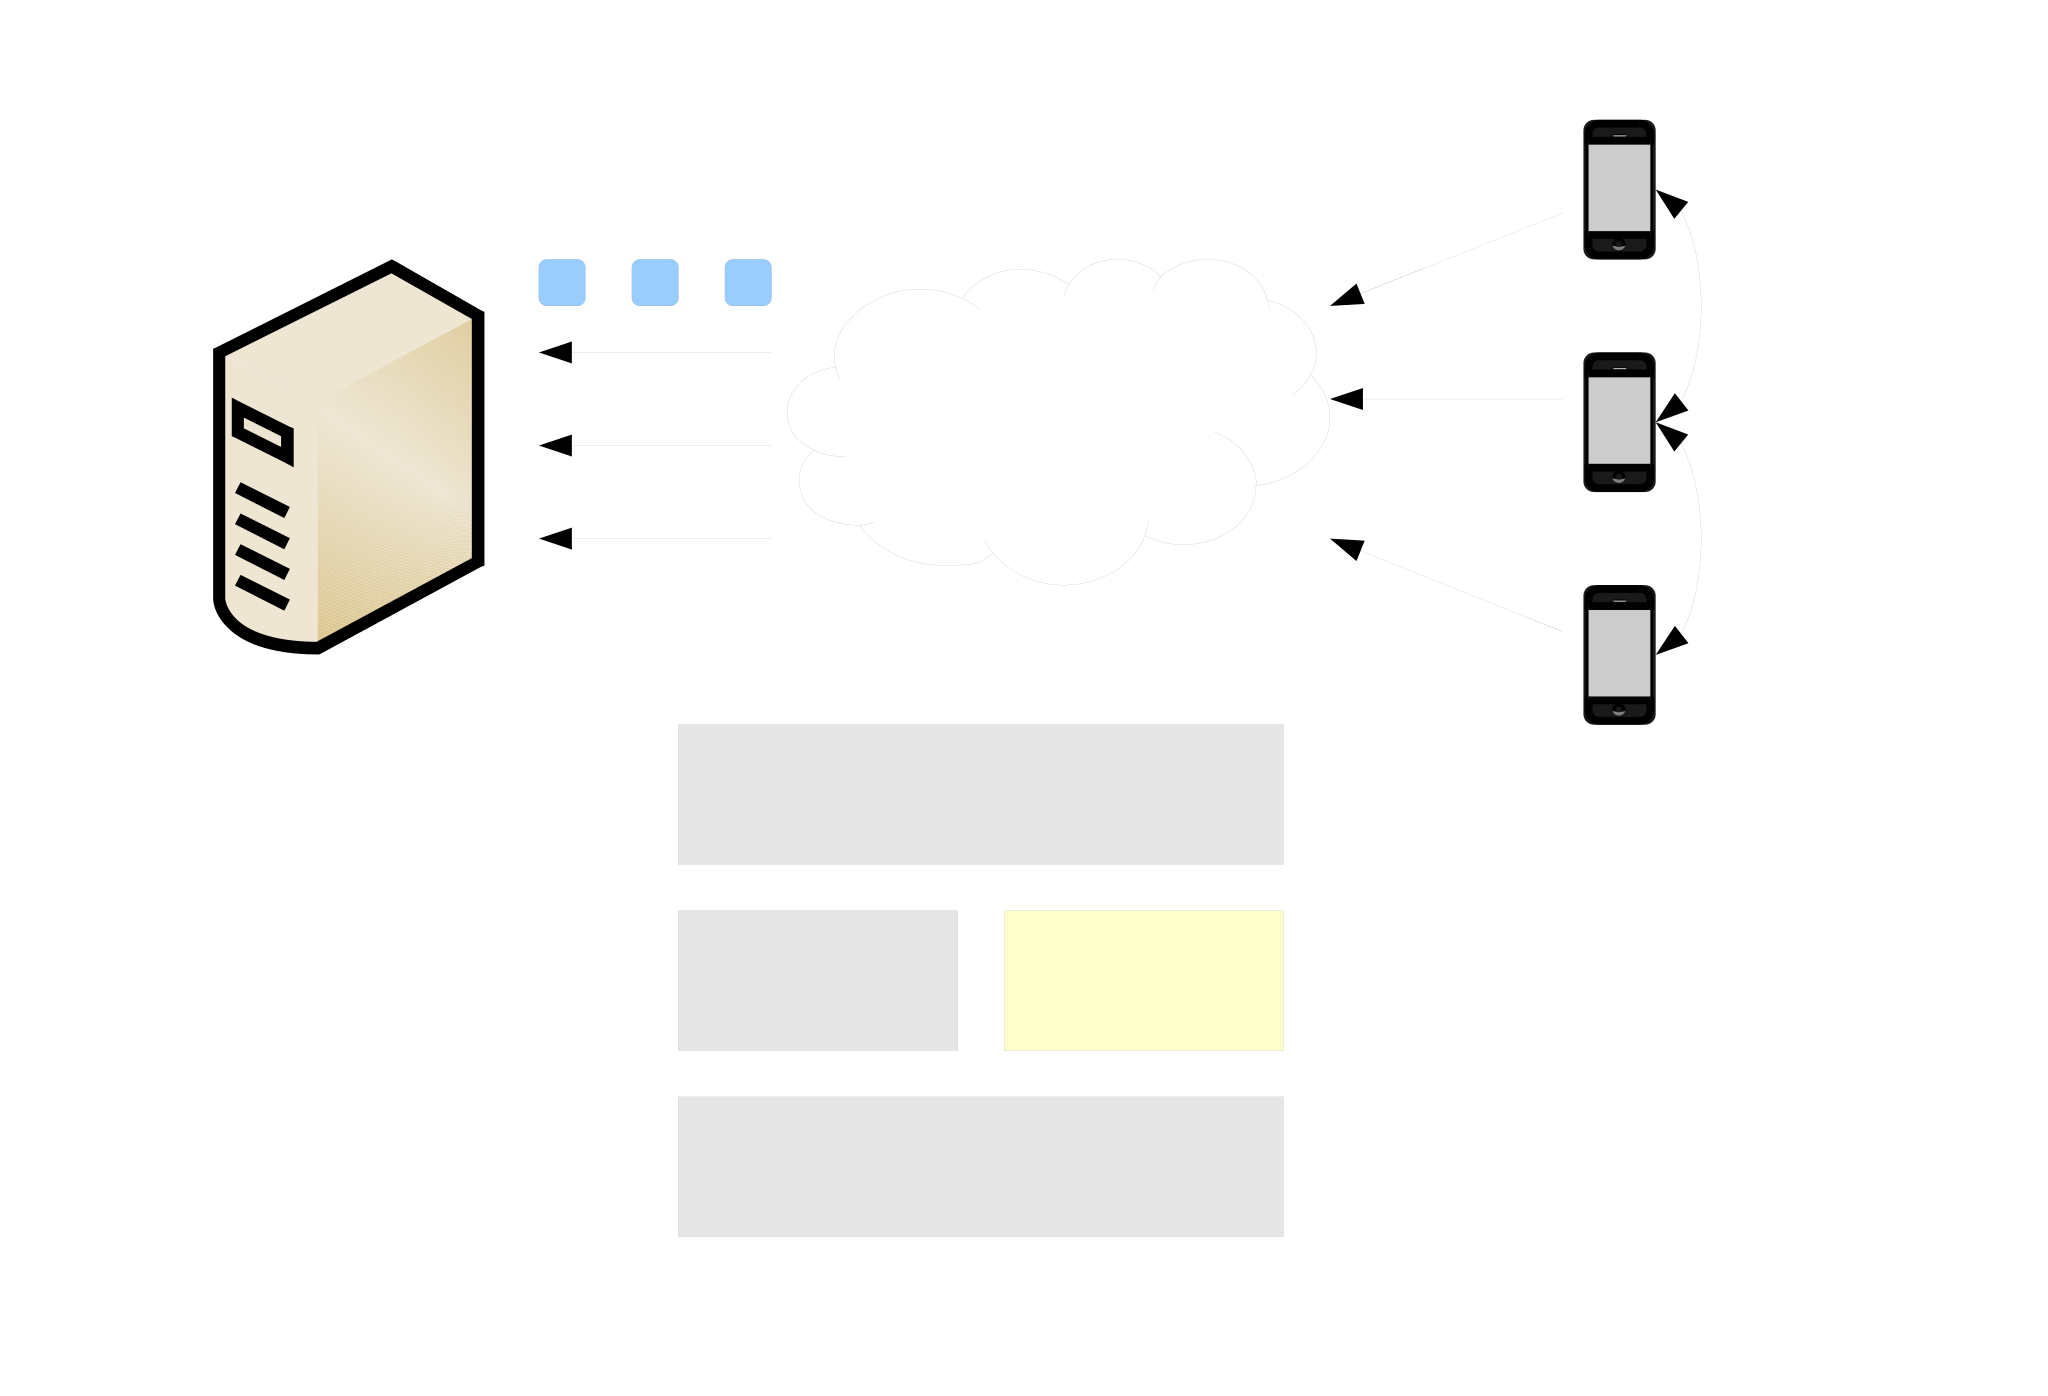
\includegraphics[width=3in]{figure1.eps}
\caption{\small \sl Anonymous Protocol.\label{fig:Stupendous}}
\end{center}
\end{figure}

What we would like is a protocol that completely removes the ownership and
source information from the data transmitted to the data collection server.
Figure 1 illustrates the concept of the theoretical anonymous One-Way
protocol.

We envision the protocol to be a network layer (layer 3) protocol that
replaces the IP protocol. The protocol will be very similar to the IP protocol
in the way that the packets includes the address of the destination host so
that the packets can be correct routed. The protocol should be able to
encapsulate upper layer (e.g. transport layer) data. The only difference is
that each packet does not include the address of the source host. In other
words, contractually, the client does not include the source address and the
server will have no access to the source information and thus keeping the
client's identity private.

Proponents might argue since the protocol resides on network layer (layer 3),
the source address could still be contained in the lower layer, e.g. the link
layer (layer 2). We argue that the source link address is different for
each hop on the route, and a route could easily contain 20 hops; therefore
the probability of tracing the link layer packet back to the original host is
really low.

%\begin{figure}[h]
%\begin{center}
%\includegraphics[width=3in]{arch.eps}
%\caption{\small \sl System Architecture.\label{fig:Stupendous}}
%\end{center}
%\end{figure}

\section{Anonymous Protocol Over Existing Protocols}\label{sec-protocol}
The One-Way protocol introduced in the previous section and Figure 1 is only
a theoretical protocol since it would take significant effort and drastic
change to current networking hardware infrastructure to introduce a new layer 3
routing protocol. In this section we modify the One-Way protocol depicted in
Figure 1 slightly so that it utilizes existing networking infrastructures. We
introduce two modifying approaches: tunneling and One-Way over User Datagram
Protocol (UDP).

\subsection{Tunneling}

In tunneling, the network topology is divided into two parts: a private
network that understands the One-Way protocol and the rest of the world that
only understand the IP protocol. The two parts are connected by the tunnel,
a special device, that does the translation between two routing protocols.

\begin{figure}[h]
\begin{center}
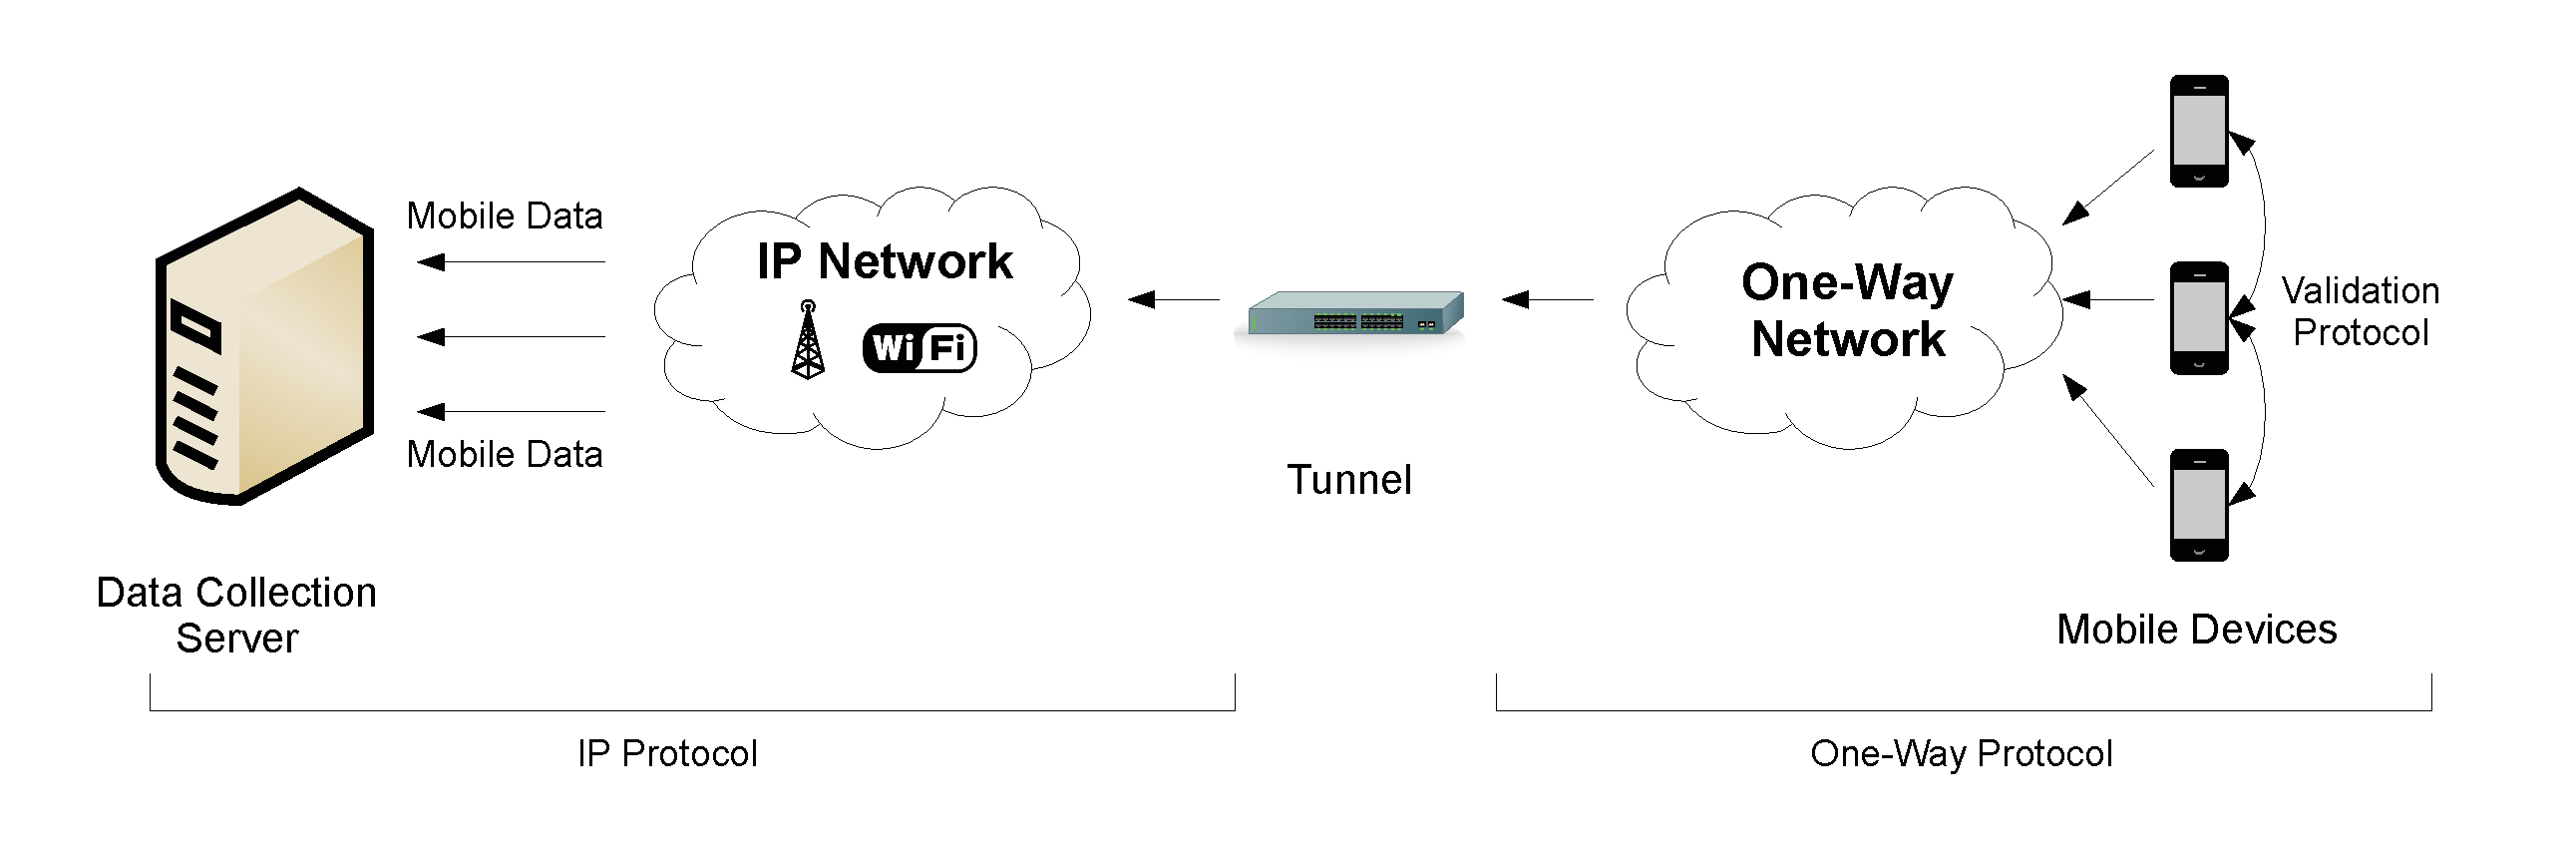
\includegraphics[width=3in]{figure2.eps}
\caption{\small \sl Tunneling.\label{fig:Stupendous}}
\end{center}
\end{figure}

\begin{figure}[h]
\begin{center}
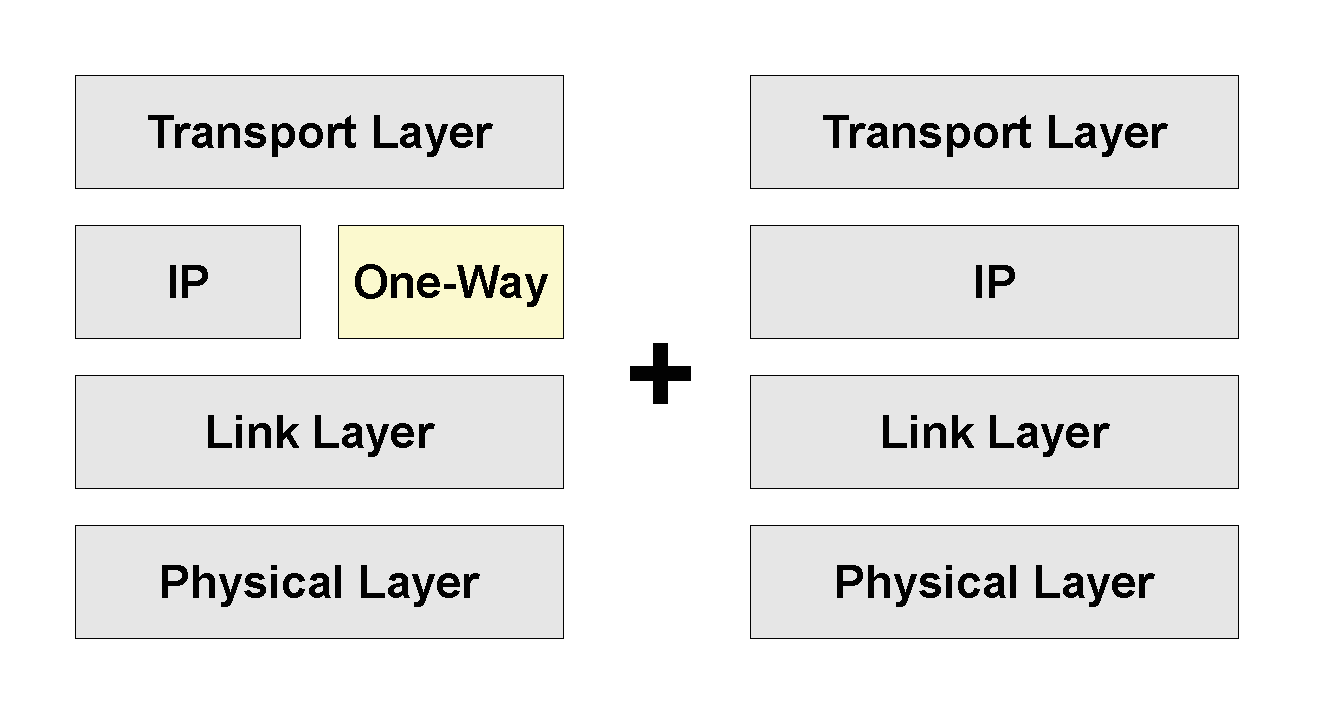
\includegraphics[width=3in]{figure2b.eps}
\caption{\small \sl Tunneling.\label{fig:Stupendous}}
\end{center}
\end{figure}

As illustrated in Figure 2, the tunneling device takes packets from the One-Way
network and forward the
data to the IP network. An important task of the tunneling device is to attach
source IP address to the packets that being forwarded. The device uses it own
IP address as the address of the packets and shields the identity of the mobile
clients. A reason for this tunneling approach is that some internet service
providers (ISP) will block packets without valid source host address. Figure 3
depicts the networking stack configuration of this approach. Tunneling is
similar to the Tor Anonymouse Protocol ~\cite{Tor}, in which clients sends data
through the designated Tor servers and the servers are responsible to deliver
the data to the destination.

Opponent could argument that attacker can still trace the mobile clients to a
specific subnet where the tunneling device resides. We argue that since most of
the clients are highly mobile, and with a number of tunneling device in one
geographic region, the identity of the mobile devices can be protected with high
confidence.

\subsection{Over User Datagram Protocol}
In this approach, we completely do away with a new routing protocol by building
the One-Way protocol as an application layer protocol on top of User Datagram
Protocol (UDP).

\begin{figure}[h]
\begin{center}
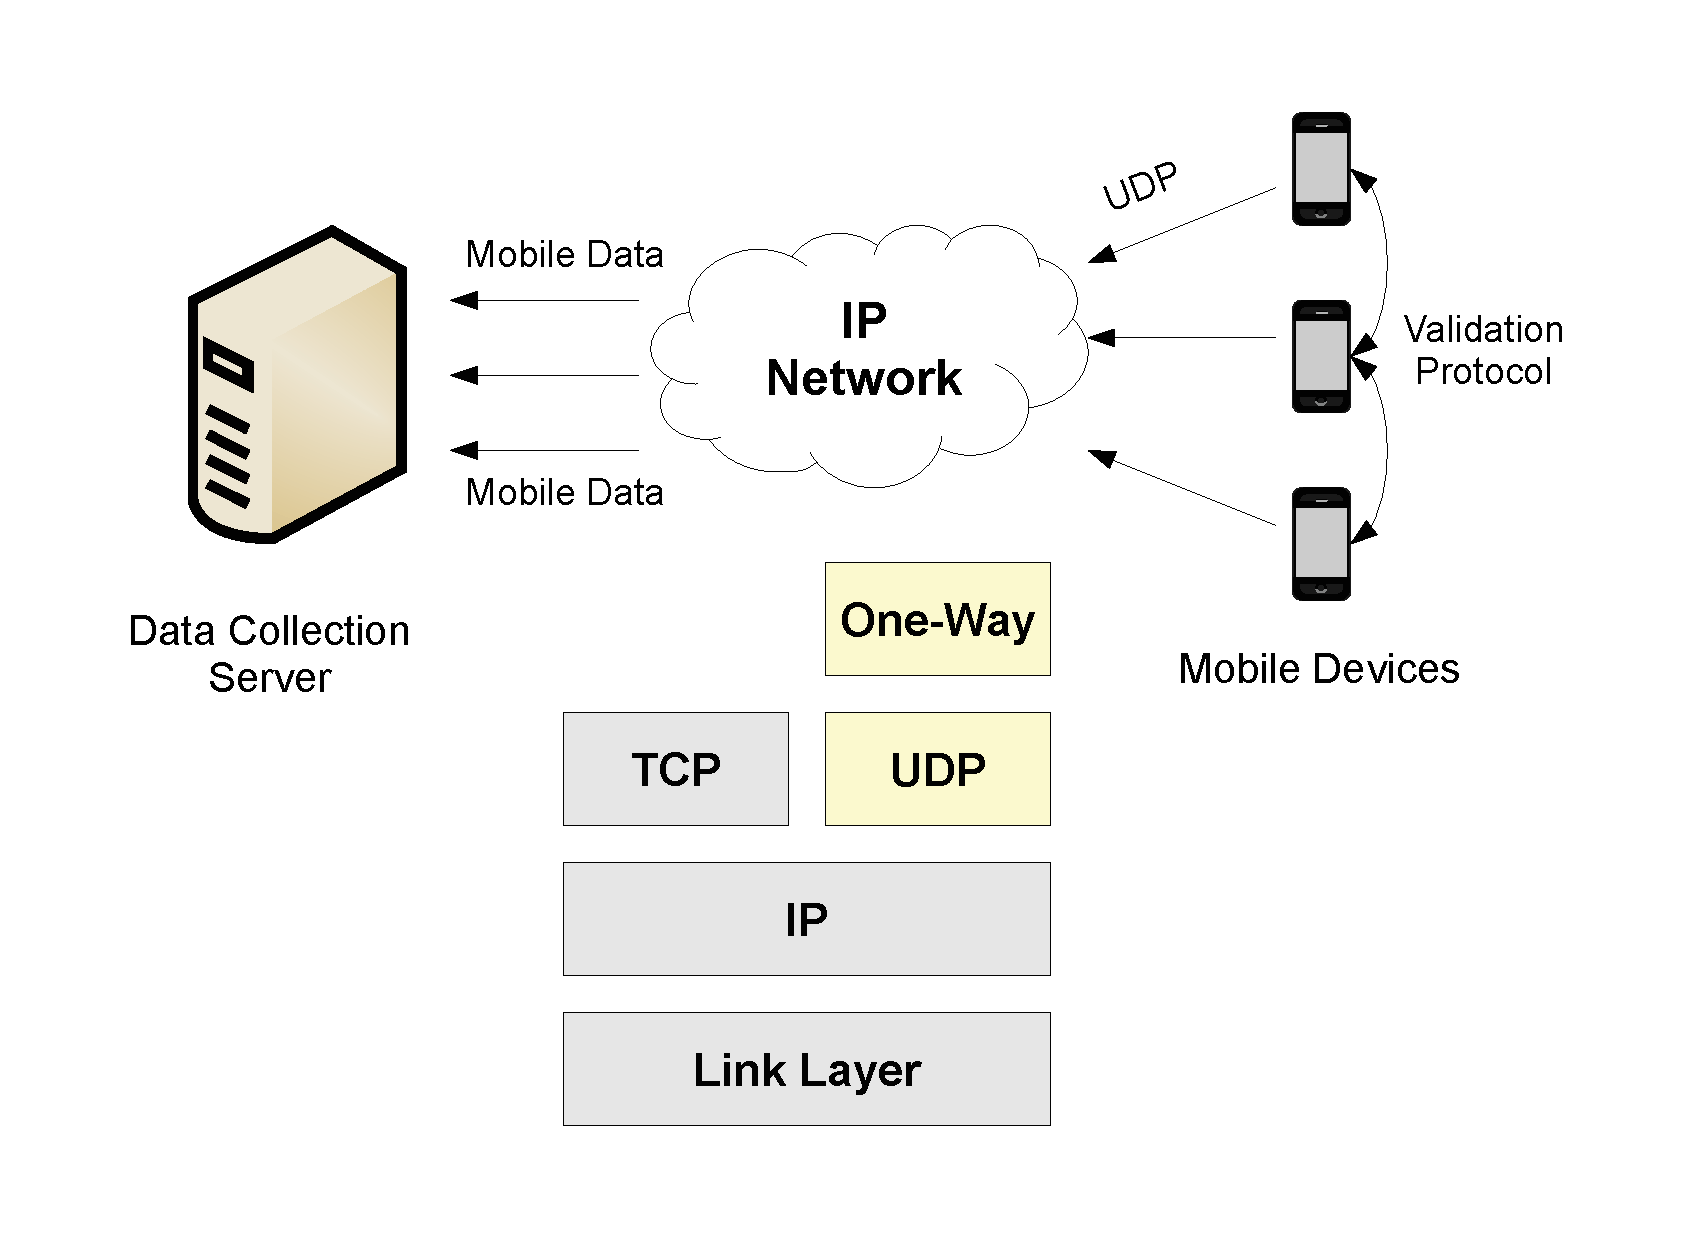
\includegraphics[width=3in]{figure4.eps}
\caption{\small \sl One-Way over UDP.\label{fig:Stupendous}}
\end{center}
\end{figure}

As illustrated in Figure 4, during transmission, the clients divides the data
into one or more UDP data packets, uses arbitrary IP address as the source
address -- to protect the identity of the mobile clients -- and sends the
packet into the network. The reason we use UDP instead of TCP is that since
the source IP is arbitrary, TCP will be unable to
establish a connection with the handshaking protocol.

In this setup, both the server and the clients need to implement the UDP One-Way
Protocol. The server has to be aware and to be able to reconstruct the complete
data from the fragments. In the future version of this protocol, we plan to
implement a protocol that allows the clients to verify that the data, in full,
has been successfully transmitted to the server.

In addition to running the protocol with no intermediate nodes, we can also combine
the UDP One-Way approach with the tunneling approach. Similar to what we described
in the previous subsection, the tunnel is an intermediate node that does translation
of protocols. The advantage of tunneling is that we can translate from UDP to TCP
protocol to provide reliable transmission. To do this kind of translation, the
tunnel create TCP packet from UDP packet and uses its own IP address as the source
address. An advantage of this translation is that the server does not necessarily
have to implement the One-Way protocol.

\subsection{Summary}
In this section we proposed an anonymous protocol that completely remove the source
address information of the data being transmitted. Three way to realize this protocol
are completely new protocol, new protocol over tunneling, and anonymous protocol
over UDP.

In the completely new protocol, we assume that we have complete freedom to implement
a new protocol and new network infrastructure. This is a very unrealistic and
impractical assumption, so we proposed new protocol and tunneling. In tunneling
we can implement the new One-Way protocol in our own small network and the tunnel
is responsible bridging our internal network and public IP network. In the UDP
approach, we build our new protocol on top of existing IP network, therefore
no new network infrastructure is required.

%In our experiment, we are able to send IP packets with arbitrary source address into
%the network and receive it on the server.


In this section, we discuss the issue of implementing the protocol proposed
in the previous section. One issue is that the Internet currently does not
support a protocol without sender information. We propose two ways of
implementing our One-Way protocol: using trusted gateways, and on top of
UDP transport layer protocol~\cite{RFC768}.

\subsection{Trust Gateway}

In the trust gateway method, we propose to implement our protocol
in hardware with a wireless access point that understands our
One-Way protocol. In the method, the network topology is divided
into two parts: a private network that understands the One-Way
protocol and the rest of the world that only understand the IP
protocol as shown in Figure~\ref{fig:gateway}. The gateway acts as
a normal wireless access point and multiplexes traffic for the
clients inside the private network.

\begin{figure}[h]
\begin{center}
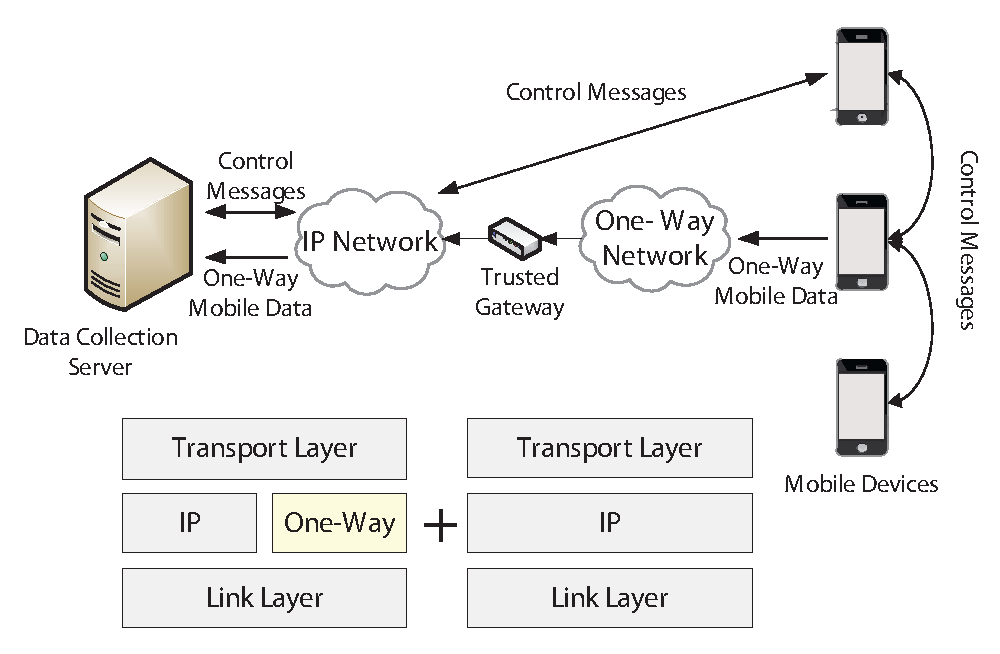
\includegraphics[width=3.4in]{one-way-gateway.eps}
\caption{Trusted Gateway.} \label{fig:gateway}
\end{center}
\end{figure}


Since the control messages do not have the issue of concealing the
sender routing address, the validation route is constructed on the
normal IP network. When a client intends to send a file to a data
collection server, she finds a peer on the traditional IP network
that runs our protocol. Afterwards, the client constructs a
connection request message and sends the message to the peer. The
first peer forwards the request to a second peer and so on until
the hop count of the request and the request is sent to the
server.

When sending payload, the sender sends payload packets through the
trusted gateway. Upon receiving a payload packet $p$, the gateway
performs a tunneling operation and transforms $p$  into a TCP
packet including all necessary information for the protocol in the
packet, using its own identity in the packet header, then forwards
the packet into the IP network. Since the gateway utilizes its own
IP address as the address of the packets, it shields the identity
of the mobile clients. One reason for this tunneling-based
approach is that some Internet service providers (ISP) block
packets without valid source host addresses.
Figure~\ref{fig:gateway} also depicts the networking stack
configuration of this approach.

Opponents of this approach may think that attackers can still
trace the mobile clients to a specific subnet where the gateway
device resides. We argue that since most of the clients are highly
mobile and with a number of access points in one geographic
region, the identity of the mobile devices can be protected with
high confidence.

\subsection{Over User Datagram Protocol}

If a subnet allows packets with anonymous sender IP addresses
(such as the broadcast address) to be forwarded through the
network, then we can build our protocol on top of existing network
protocols. In this approach, we completely do away with trusted
access points by building the One-Way protocol as an application
layer protocol on top of the User Datagram Protocol (UDP) and
employ existing network hardware and infrastructure. This method
is illustrated in Figure~\ref{fig:imp-udp}.

\begin{figure}[h]
\begin{center}
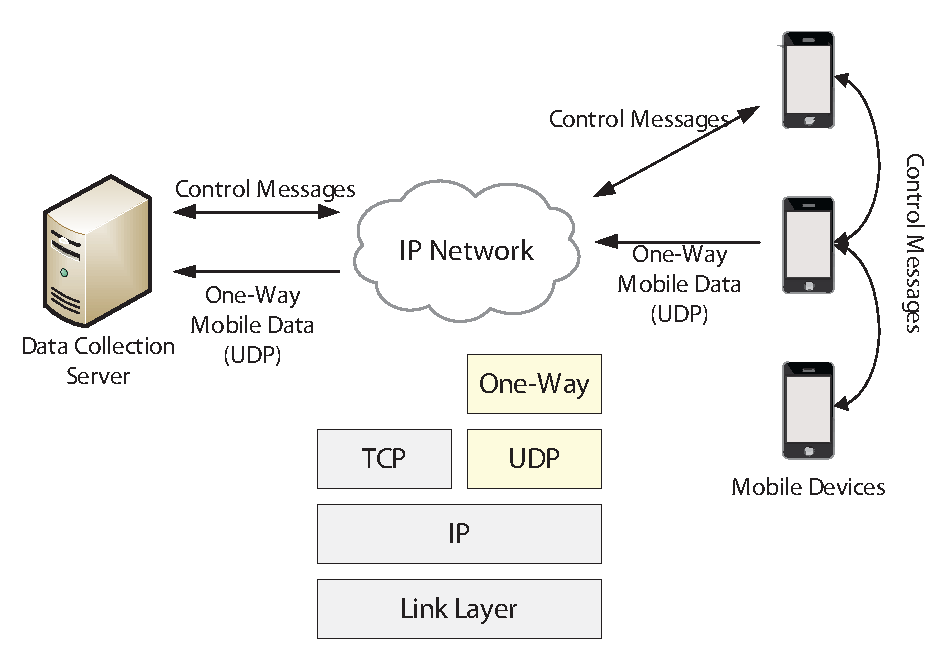
\includegraphics[width=3.4in]{one-way-udp.eps}
\caption{One-Way over UDP.} \label{fig:imp-udp}
\end{center}
\end{figure}

The steps for making a connection request is the same for the
trusted gateway approach, but payload transmission is slightly
different. During payload transmission, instead of letting a
gateway to replace the identity of the packets, the sender uses
the broadcast IP address (255.255.255.255) in the sender address
field of the packet. This denotes that the sender is anonymous and
the server should treat the data transmission using anonymous
protocol.

Note that the reason we use UDP is that TCP will not work in our
approach because it is a connection oriented protocol. With an
arbitrary IP address field, TCP will be unable to establish a
connection with the handshaking protocol.

%In our experiment, we are able to send IP packets with arbitrary source address into
%the network and receive it on the server.

\section{Attack Models}\label{sec-attack}

In this section we consider several attack models and discuss how our
design offer protection against these attacks.

\subsection{Server Attack}
The first attack model is server attack. In this attack, the server cannot
be trusted or can be a source of identity of disclosure. Most services logs
the identity of the users with the data submitted through their services.
If the server is malicious, or mandated by someone powerful for disclosure,
privacy of the users are compromised.

First we analyze the payload transmission part of our design against
server attack. We assume that the server can see the packets sent to it,
but does not see the packets in the network before it reaches it. In
other words the server does not control the Internet and cannot perform
traffic analysis on the Internet. Under this assumption, in our One-Way
protocol the sender has the anonymity level of beyond suspicion since
a server cannot infer any identity information from the data packet it
receives. The only linking information is the identity of the network
device (e.g. link layer switch) at the last hop of the route. We assume
the service does not control the Internet, therefore it cannot link
this information back to the sender.

Next we analyze our validation protocol again server attack. Keep in mind,
our validation uses peer network to transmit acknowledgement and control
messages.
Since the server has to run our anonymous validation protocol, it is
consider one of the network peers and therefore it can
find out the users in the peer network, but the server does not know the
original hop count $h$ of the control packets. In addition, any peer can
potentially be connected with any other peers therefore, the sender is
also beyond suspicion in this case.

\subsection{Eavesdrop and Traffic Analysis}

In eavesdrop attack, we assume that the data transmission route is divided
into segments each controlled by a network administrator. An attacker is
able to listen to the traffic of a segment, but cannot eavesdrop
on all the network segments of the route. In other words, the attacker
not have the full view of the entire route, but only a segment.

There are two scenarios. The first scenario is that the sender of the
data does not reside on the network on which the attacker is eavesdropping
and the the level of anonymity for the sender is beyond suspicion. Although
the attacker is able to listen to the traffic to his network, it is
unable to see who the sender is from the other network.

The second scenario is that the sender and the attacker are on the same
network. In this case the attacker is able to analyze the traffic of any
node on the network. In this scenario, our design is unable to protect the
identity of the sender and the level of anonymity is exposed. The way the
attack could get the sender's identity is to compare the incoming and
outgoing traffic for every node in the network. For the nodes that have
outgoing traffic for a specific content without corresponding incoming
traffic is suspected of data originator. Encryption of data on top of our
design can mitigate this attack.

\section{Performance Evaluation}\label{sec-evaluation}

In this section we present our performance evaluation results.

\subsection{Transmission Overhead}

Transmission overhead is ratio between the amount of additional data that
is imposed by a protocol to the effective data transmitted. In our
measurements, transmission overhead include the headers of a protocol for
each packets as well as any replication of the data to peers. Let $D$ be
the original data captured by a mobile device to be sent to the server and
$D'$ be the total 
 


\subsection{Transmission Latency}
%\section{Query Processing}\label{sec-processing}
%\input{processing}

\section{Future Work}
Future work includes reliability and security of this approach.


%\section{Demonstration}\label{sec-demo}
%\input{demo}

\section{Conclusions}\label{sec-conc}

Due to the growth of the number and power of mobile phones, participatory
sensing is a new growing area in computer science. The potential of this
research is great

Due to being a new area, many issues are unaddress, including the identity
privacy of the participants. In this paper we presented an approach to privacy
protection by introducing One-Way anonymous protocol in which we remove
the source information of the data from the data transmitted to the server.

We first presented the protocol in the most theoretical form. The protocol
is a routing protocol that does not include the source host address. Since
The protocol cannot be realized with the existing networking infrastructure,
we introduced two modification to the protocol. The first modification is
to use a tunnel forward the packet from the One-Way network to the rest of
the Internet, where the server resides.

The second approach is to build the One-Way an application protocol on top
of UDP. In this approach we used arbitrary address as the source address to
conceal mobile client's identity. 

\section*{Acknowledgment}

The heading of the Acknowledgment section and the References section
must not be numbered.

Causal Productions wishes to acknowledge Michael Shell and other
contributors for developing and maintaining the IEEE LaTeX style files
which have been used in the preparation of this template.  To see the
list of contributors, please refer to the top of file IEEETran.cls in
the IEEE LaTeX distribution.

\bibliographystyle{abbrv}
\bibliography{bib}

\end{document}
